\documentclass{article}
\usepackage[utf8]{inputenc}
\usepackage{graphicx}
\graphicspath{{images/}}
\DeclareGraphicsExtensions{.pdf,.png,.jpg}
%Russian-specific packages
%--------------------------------------
\usepackage[T2A]{fontenc}
\usepackage[utf8]{inputenc}
\usepackage[russian]{babel}
\usepackage{amssymb}
\usepackage{color}
\usepackage[left=10mm, top=10mm, right=5mm, bottom=10mm, nohead, nofoot]{geometry}
%--------------------------------------
\title{Лабораторная работа №1.3.3 \\ Определение вязкости воздуха по скорости течения через тонкие трубки.}
\author{Павлов Дмитрий}
\date{Апрель 2018}

\begin{document}

\maketitle
\begin{center}
Долгопрудный \\2018
\end{center}
\newpage

\newpage
\section{Предисловие}
\textbf{Цель работы:} экспериментально выявить участок сформированного течения, определить режимы ламинарного и турбулентного течения; определить число Рейнольдса.\\
\\
\textbf{В работе используются:} металлические трубки, укрепленные на горизонтальной подставке; газовый счетчик; микроманометр типа ММН; стеклянная U-образная трубка; секундомер.\\
\\
При малых скоростях потока движение оказывается ламинарным (слоистым), скорости частиц меняются по радиусу и направлены вдоль оси трубки. С увеличением скорости потока движение становится турбулентным, и слои перемешиваются. При турбулентном движении скорость в каждой точке быстро меняет величину и направление, сохраняется только средняя величина скорости.\\
Характер движения газа (или жидкости) в трубке определяется безразмерным числом Рейнольдса:
\begin{center}
    $Re = \frac{vr\rho}{\eta}$
\end{center}  
где $v$ — скорость потока,\\
$r$ — радиус трубки,\\
$\rho$ — плотность движущейся среды, \\
$\eta$ — ее вязкость.\\
В гладких трубах круглого сечения переход от ламинарного движения к турбулентному происходит при Re $\approx$ 1000.\\
\\
При ламинарном течении объем газа $V$ , протекающий за время $t$ по трубе длиной $l$, определяется формулой Пуазейля:
\begin{center} \large{
    $Q_V = \frac{\pi r^4}{8l \eta}\Delta P$}
\end{center} 
Отметим условия, при которых справедлива формула (2). Прежде всего необходимо, чтобы с достаточным запасом выполнялось неравенство Re < 1000. При втекании газа в трубку из большого резервуара скорости слоев вначале постоянны по всему сечению.\begin{center} 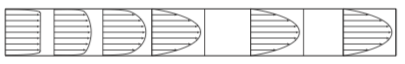
\includegraphics[scale = 0.75]{q5.png} \end{center}  По мере продвижения газа по трубке картина распределения скоростей меняется, так как сила трения о стенку тормозит прилежащие к ней слои. Характерное для ламинарного течения параболическое распределение скоростей устанавливается на некотором расстоянии $a$ от входа в трубку, которое зависит от радиуса трубки $r$ и числа Рейнольдса по формуле:
\begin{center}
    $a=0.2r \cdot Re$
\end{center}  
\textbf{Экспериментальная установка}
\begin{center} 
    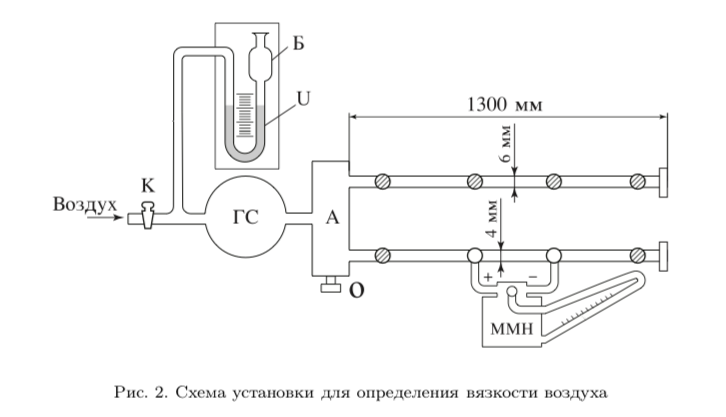
\includegraphics[scale = 0.5]{q6.png} 
\end{center}
\section{Ламинарное течение.}
    Оценим расстояние на котором происходит формирование потока при ламинарном течении по формуле: 
    \begin{equation}
        a=0.2r \cdot Re
    \end{equation}
    где $r$ - радиус сечения трубки\\
    Re - число Рейнольдса, для оценки возьмем его равным 1000.\\
    $a = 0.2r \cdot Re = 0.2 \cdot (0.5 \cdot 3.9mm)  \cdot 1000 = 39cm$

\section{Вязкость воздуха.}
    \subsection{Измерение зависимости падения давления от расхода воздуха.}
    \begin{center}
        \begin{tabular}{ | l | l | l | l | l | l |}
            \hline
            $\Delta P$, ед. шкалы & $\Delta P$, Па & $\Delta V$, л  & $\Delta t$, с &  Q, л/c & Q, м/с \\ \hline
            16  & 31.38  & 2.5 & 127 & 0.0197 & 0.000020 \\
            30  & 58.84  & 7.5 & 206 & 0.0364 & 0.000036 \\
            39  & 76.49  & 7.5 & 155 & 0.0484 & 0.000048 \\
            65  & 127.49 & 10  & 122 & 0.0820 & 0.000082 \\
            80  & 156.91 & 15  & 152 & 0.0987 & 0.000099 \\
            96  & 188.29 & 15  & 141 & 0.1064 & 0.000106 \\
            124 & 243.20 & 10  & 90  & 0.1111 & 0.000111 \\
            153 & 300.08 & 10  & 84  & 0.1190 & 0.000119 \\
            174 & 341.27 & 25  & 200 & 0.0125 & 0.000125 \\
            205 & 402.07 & 10  & 76  & 0.1316 & 0.000132 \\
            261 & 511.90 & 25  & 162 & 0.1543 & 0.000154 \\
            \hline
        \end{tabular}\\
        Результаты измерения зависимости падения давления в трубке от расхода воздуха.
    \end{center}
    $\Delta P$ - падение давления\\
    $\Delta V$ - объем воздуха\\
    $\Delta t$ - время, за которое прошло V литров воздуха\\
    $Q$ - расход воздуха, $Q=\frac{\Delta V}{\Delta t}$
    \subsection{По данным таблицы построим график $P(Q)$:}
        Используем данные, при которых течение воздуха в трубке ламинарное (до 200 Па)
    \begin{center}
        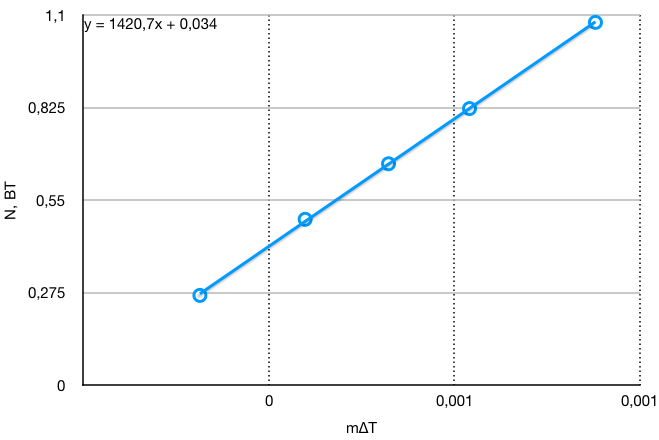
\includegraphics[scale = 0.5]{q1.png}\\
        График зависимости падения давления в трубке от расхода воздуха.
    \end{center}
    График линеен, что соответсвует формуле Пуазейля:
    \begin{equation}
        Q = \frac{\pi R^4}{8 \eta l} \Delta P
    \end{equation}
    \newpage
    Из коэффициент наклона графика и уравнения (2) можем найти вязкость воздуха:
    \begin{equation}
        \eta = \frac{\pi R^4}{8lk},
    \end{equation}
    \begin{center}
        $k = \Delta Q/ \Delta P = 1.7\cdot10^6$ - коэффициент наклона прямой.
    \end{center}
    Итого, коэффициент вязкости воздуха равен:\\
    \begin{center}
        $\eta = \frac{\pi R^4}{8lk} = \frac{3.14 \cdot (0.5 \cdot 39mm)^4}{8 \cdot 50cm \cdot 1.7 \cdot 10^6} = 1.9 \cdot 10^{-5}$ кг $\cdot$ м /с
    \end{center}
    \subsection{Погрешности}
        \begin{center}
            $\frac{\sigma_\eta}{\eta} = \sqrt{(\frac{\sigma_\frac{\Delta P}{Q}}{\frac{\Delta P}{Q}})^2 + 4(\frac{\sigma_n}{r})^2 + (\frac{\sigma_l}{l})^2} = \sqrt{0.01^2 + 4 \cdot 0.01^2 + 0.01^2} = 0.024 \approx 2.5\%$
        \end{center}
    Погрешность измерения складывается из погрешностей измерения длины трубки:
    \begin{center}
        $\sigma_l$ = 0.5 см\\
        $l$ = 50 см\\
        $\epsilon_l$ = 0.01
    \end{center}
    из погрешностей измерения радиуса трубки:
    \begin{center}
        $\sigma_r$ = 0.05 мм\\
        $r$ = 3.9 мм\\
        $\epsilon_r$ = 0.01
    \end{center}
    и из погрешности определения наклона графика:
    \begin{center}
        k = $1.7 \cdot 10^{-6} \pm 1.26 \cdot 10^{-8}$\\
        $\epsilon_k = 0.01$
    \end{center}
\section{Число Рейнольдса.}
    \subsection{Вычисление.}
        Вычислим значение числа Рейнольдса для переходной области между ламинарным и турбулентным течениями.
        \begin{center}
            $Re = \frac{Qnp}{s\eta} = 1211$
        \end{center}
    \subsection{Погрешности}
        \begin{center}
            $\frac{\sigma_Re}{Re} = \sqrt{(\frac{\sigma_Q}{Q})^2 + (\frac{\sigma_r}{r})^2 + (\frac{\sigma_\eta}{\eta})^2} = 0.1 = 10\%$
        \end{center}
    Погрешность измерения складывается из погрешностей вязкости воздуха:
    \begin{center}
        $\epsilon_\eta$ = 0.024 (см. п. 3.3)
    \end{center}
    из погрешностей измерения радиуса трубки:
    \begin{center}
        $\sigma_r$ = 0.05 мм\\
        $r$ = 3.9 мм\\
        $\epsilon_r$ = 0.01
    \end{center}
    и из погрешности определения расхода воздуха:
    \begin{center}
        $\epsilon_Q = 0.1$
    \end{center}
\section{Экспериментальное определение расстояния на котором устанавливается ламинарное течение.}
    \subsection{Измерение зависимости падения давления от длины трубки.}
    \begin{center}
        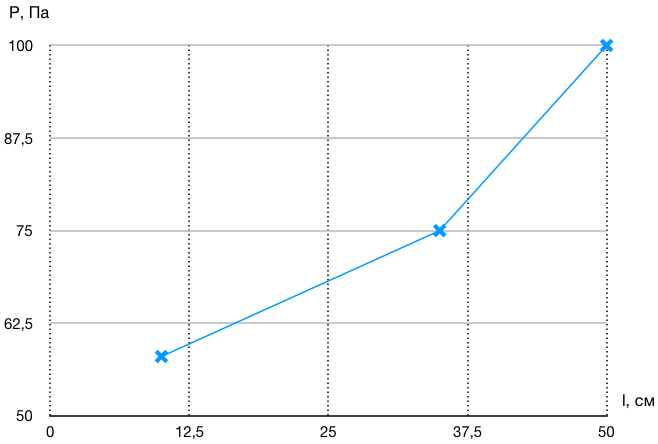
\includegraphics[scale = 0.5]{q3.png}\\
        График зависимости падения давления в трубке от длины трубки.
    \end{center}
    Из графика видно, что ламинарное течение устанавливается на 35 см.\\
    Результаты расчета (п. 2) и измерения совпали.
\section{Проверка формулы Пуазейля.}
    \subsection{Для всех трубок на участках со сформированным течением снимем зависимости $Q = f(P)$.}
    \begin{center}
        \begin{tabular}{ | l | l | l | l | l |}
            \hline
            d, мм & l, см & $\frac{\Delta Q}{\Delta P}$ & $\ln \frac{8l \eta Q}{\pi \Delta P}$ & $\ln r$ \\ \hline
            3.9 & 50 & $5.4 \dot 10^{-7}$ & -25.3  & -6.3 \\
            3   & 30 & $3.4 \dot 10^{-7}$ & -26.4  & -6.5 \\
            5.2 & 50 & $1.2 \dot 10^{-6}$ & -24.58 & -6.0 \\
            \hline
        \end{tabular}
    \end{center}
    d - диаметр трубки \\
    l - длина трубки \\
    r - радиус трубки
    \subsection{Построим график, по оси ординат $ln(\frac{8l \eta Q}{\pi \Delta P})$, по оси абсцисс $ln(r)$}
    \begin{center}
        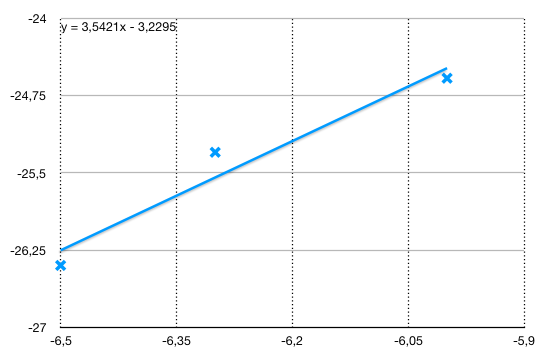
\includegraphics[scale = 0.5]{q4.png}\\
        График зависимости $\frac{8l \eta Q}{\pi \Delta P}$ от $r$ в логарифмическом масштабе.
    \end{center}   
    Коэффициент наклона графика оказался равен 3.6, что немного ниже ожидаемого значения k = 4, соответствующего степени n в формуле Пуазейля.
    \subsection{Погрешности:}
    При помощи МНК вычисляем ошибку коэффициента наклона прямой:
    \begin{center}
        $\sigma_k \approx 0.5$\\
        $\epsilon_k = 10\%$
    \end{center}   
    То есть ожидаемый результат (k = 4) лежит в пределах погрешности.
\section{Вывод}
Определили коэффициент вязкости воздуха:\\
$\eta = (19 \pm 0.5) \cdot 10^{-4}$ кг $\cdot$ м /с\\
$\epsilon_\eta = 2.5 \%$\\
Определили число Рейнольдса для данной трубки:\\
$Re = 1211 \pm  10$\\
$\epsilon_{Re} = 10\%$\\
Проверили формулу Пуазейля, значение радиуса трубки находится в формуле в 4-й степени.
\end{document}
